\section{Axial wave propagation in coupled nanorod system with nonlocal small scale effects}
As we have seen, the stress-strain relation for a rod can be written as eq.\eqref{onedimconst}, or:\\
\begin{equation}
\sigma_{xx} = g^2 \frac{\partial^2 \sigma_{xx}}{\partial x^2} = E \varepsilon_{xx} = E \frac{\partial u}{\partial x}
\end{equation}
where $E$ is the modulus of elasticity,$\sigma_{xx}$ and $\varepsilon_{xx}$ are the local stress
and strain components in the $x$ direction, respectively, and $g=e_0 a$ nonlocal scaling parameter. The equation
of motion for an axial rod can be obtained as\\
\begin{equation}
\dfrac{\partial N}{\partial x} +f(x,t) =\rho A \dfrac{\partial^2 u}{\partial t^2}
\end{equation}
where $f(x, t)$ is the axially distributed force per unit length and $N$ is
the stress resultant for local or classical elasticity and is defined by\\
\[N = \int_A \sigma_{xx} dA\]
This can be simplified to:\\
\begin{equation}
EA \dfrac{\partial^2 u}{\partial x^2} + g^2 \rho A \dfrac{\partial^4 u}{\partial x^2 \partial t^2} - \rho A \dfrac{\partial^2 u}{\partial t^2} + f - g^2 \dfrac{\partial^2 f}{\partial x^2}
\end{equation}
Hence, if the longitudinal displacements are $u_1(x,t)\text{ and } u_2(x,t)$, the governing equations of the axial wave propagation of DNRS
can be expressed as\\
\begin{equation}
E_1A_1 \dfrac{\partial^2 u_1}{\partial x^2} + g^2 \rho A \dfrac{\partial^4 u_1}{\partial x^2 \partial t^2} - \rho A \dfrac{\partial^2 u_1}{\partial t^2} + f_1 - g^2 \dfrac{\partial^2 f_1}{\partial x^2}
\end{equation}
\begin{equation}
E_2A_2 \dfrac{\partial^2 u_2}{\partial x^2} + g^2 \rho A \dfrac{\partial^4 u_2}{\partial x^2 \partial t^2} - \rho A \dfrac{\partial^2 u_2}{\partial t^2} + f_2 - g^2 \dfrac{\partial^2 f_2}{\partial x^2}
\end{equation}
Here the distributed forces $f_1\text{ and } f_2$ on nanorod-1 and nanorod-2 are given
as\\
\begin{equation}
f_1 = K_{CS} (u_2 - u_1)
\end{equation}
\begin{equation}
f_2 = K_{CS} (u_1 - u_2)
\end{equation}
Substituting these forces in the governing equations give:\\
\begin{multline}
E_1A_1 \dfrac{\partial^2 u_1}{\partial x^2} + g^2 \rho A \dfrac{\partial^4 u_1}{\partial x^2 \partial t^2} - \rho A \dfrac{\partial^2 u_1}{\partial t^2} \\+ K_{CS} (u_2 - u_1) - g^2 K_{CS} \left( \dfrac{\partial^2 u_2}{\partial x^2} - \dfrac{\partial^2 u_1}{\partial x^2}\right) = 0
\end{multline}
\begin{multline}
E_2A_2 \dfrac{\partial^2 u_2}{\partial x^2} + g^2 \rho A \dfrac{\partial^4 u_2}{\partial x^2 \partial t^2} - \rho A \dfrac{\partial^2 u_2}{\partial t^2} \\ - K_{CS} (u_2 - u_1)  + g^2 K_{CS} \left( \dfrac{\partial^2 u_2}{\partial x^2} - \dfrac{\partial^2 u_1}{\partial x^2}\right) = 0 
\end{multline}
Using a linear harmonic solution as in eq. \eqref{harmonicsoln}, we can obtain the dispersion relation as:\\
\[
\begin{bmatrix}
Z_{11} & Z_{12} \\
Z_{21} & Z_{22} 
\end{bmatrix}
\begin{Bmatrix}
\hat{u_1}\\
\hat{u_2}
\end{Bmatrix} = 
\begin{Bmatrix}
0\\
0
\end{Bmatrix}
\]
which yields\\
\begin{equation}
(C_1 C_5 - C_3^2)k^4 - (C_1 C_6 + C_2 C_5 - 2 C_3 C_4) k^2 + C_2 C_6 - C_4^2 = 0
\label{dispeqn}
\end{equation}
where $C_1=-E_1A_1 + \rho_1 A_1 g^2 \omega^2\text{, } C_2=\rho_1 A_1 g^2 \omega^2 - K_{CS} \text{, } C_3=K_{CS} g^2\text{, } C_4 =K_{CS}\text{, }C_5=-E_2 A_2+\rho_2 A_2 g^2 \omega^2 - K_{CS}g^2\text{ and }C_6=\rho_2 A_2 \omega^2-K_{CS}$
The wavenumber is a function of wave frequency, the nonlocal
scaling parameter $g$ and the material and geometrical properties of
the nanorod. If $g = 0$, the wavenumber is directly proportional to
wave frequency, which will give a non-dispersive wave behavior.
\begin{figure}
\centering
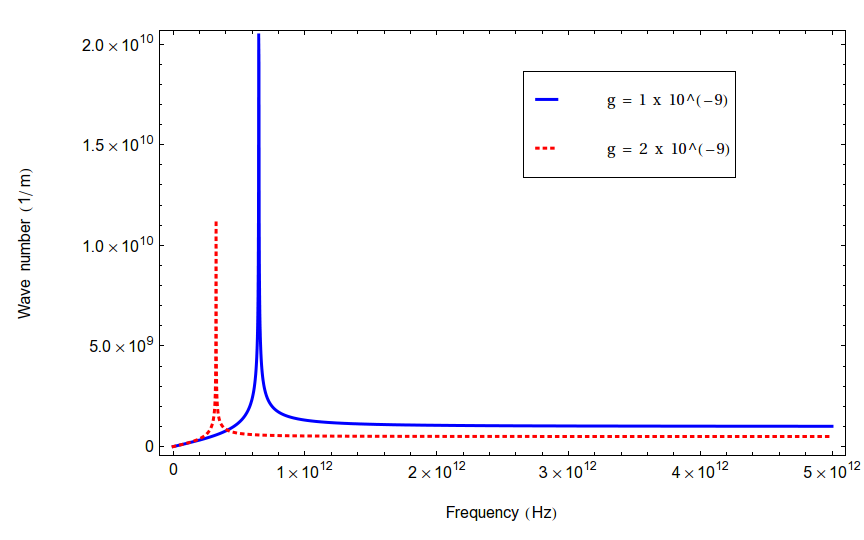
\includegraphics[scale=0.5]{dnrs_disp}
\end{figure}
\subsection*{Computation of cut-off frequency}
In the wavenumber dispersion curves, the frequency at which
the imaginary part of the wavenumber becomes real is called as
the frequency band gap region $0-\omega_{cut}$ The expression for fre-
quency band gap is obtained by setting k = 0 in dispersion relation \eqref{dispeqn}. by setting $k = 0$, i.e., solving $C_2 C_6- C_4^2 =0$, we get the cut-off frequency as\\
\begin{equation}
\omega_{cut}=\sqrt{K_{CS}\left[\dfrac{1}{\rho_1 A_1} + \dfrac{1}{\rho_2 A_2}\right]}
\end{equation}

